\documentclass[12pt]{article}

\usepackage{tikz}
\usetikzlibrary{graphs,quotes,arrows.meta}
\usetikzlibrary{automata,positioning}
\usetikzlibrary{shapes,arrows}
\usepackage{amsmath, amssymb}
\usetikzlibrary{chains}
\usetikzlibrary{matrix,backgrounds}
\usetikzlibrary{calc}



\newcommand{\chainlabel}[2]{\path [<-, draw, shorten >=10pt] (#1) |- node [at end] {#2} ++(-1,1);}

\begin{document}


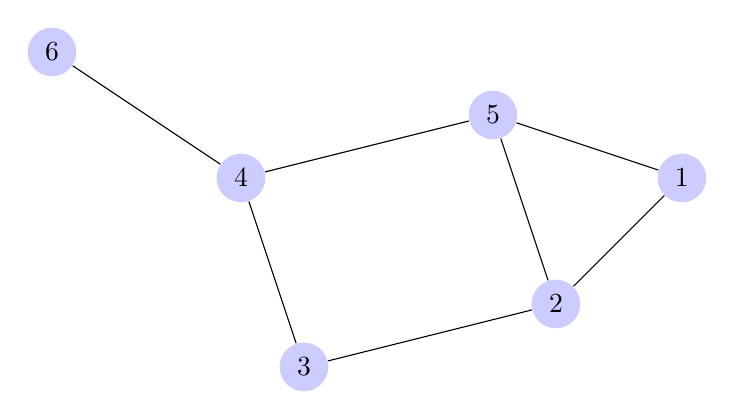
\begin{tikzpicture}
  [scale=.8,auto=left,every node/.style={circle,fill=blue!20}]
  \node (n6) at (1,10) {6};
  \node (n4) at (4,8)  {4};
  \node (n5) at (8,9)  {5};
  \node (n1) at (11,8) {1};
  \node (n2) at (9,6)  {2};
  \node (n3) at (5,5)  {3};

  \foreach \from/\to in {n6/n4, n4/n5, n5/n1, n1/n2, n2/n5, n2/n3, n3/n4}
    \draw (\from) -- (\to);
\end{tikzpicture}




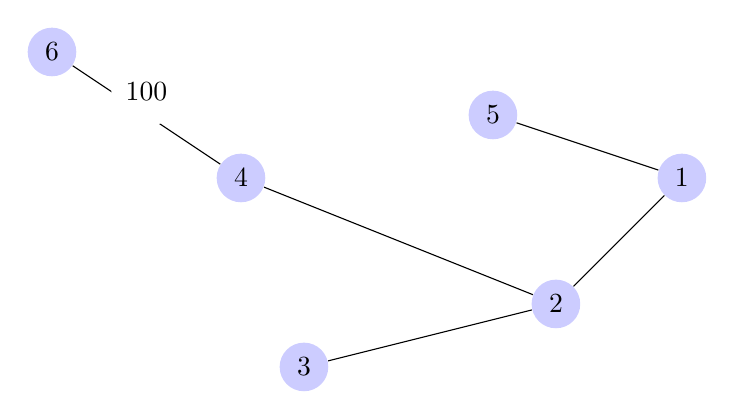
\begin{tikzpicture}
  [scale=.8,auto=left,every node/.style={circle,fill=blue!20}]
  \tikzstyle{v}=[circle,minimum size=1mm,fill=transparent!0]
  \node (n6) at (1,10) {6};
  \node (n4) at (4,8)  {4};
  \node (n5) at (8,9)  {5};
  \node (n1) at (11,8) {1};
  \node (n2) at (9,6)  {2};
  \node (n3) at (5,5)  {3};
  
  \draw (n6) node[v,xshift=1.2cm,yshift=-.5cm] {100} -- (n4);
  \draw (n4) -- (n2);
  \draw (n2) -- (n1);
  \draw (n1) -- (n5);
  \draw (n2) -- (n3);
\end{tikzpicture}






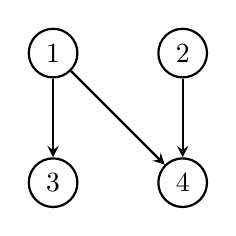
\begin{tikzpicture}[xscale=1,yscale=1,>=stealth]
\tikzstyle{v}=[circle,minimum size=1mm,draw,thick]
\node[v] (a) {$1$};
\node[v] (b) [right=of a] {$2$};
\node[v] (c) [below=of a] {$3$};
\node[v] (d) [below=of b] {$4$};
\draw[thick,->] (a) to node {} (c);
\draw[thick,->] (a) to node {} (d);
\draw[thick,->] (b) to node {} (d);
\end{tikzpicture}





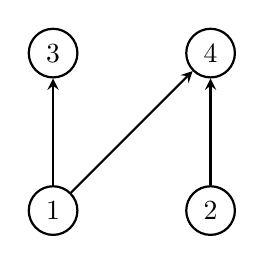
\begin{tikzpicture}[xscale=1,yscale=1,>=stealth]
\tikzstyle{v}=[circle,minimum size=1mm,draw,thick]
\node[v] (a) at (0,0) {$1$};
\node[v] (b) at (2,0) {$2$};
\node[v] (c) at (0,2) {$3$};
\node[v] (d) at (2,2) {$4$};
\draw[thick,->] (a) to node {} (c);
\draw[thick,->] (a) to node {} (d);
\draw[thick,->] (b) to node {} (d);
\end{tikzpicture}










\begin{center}
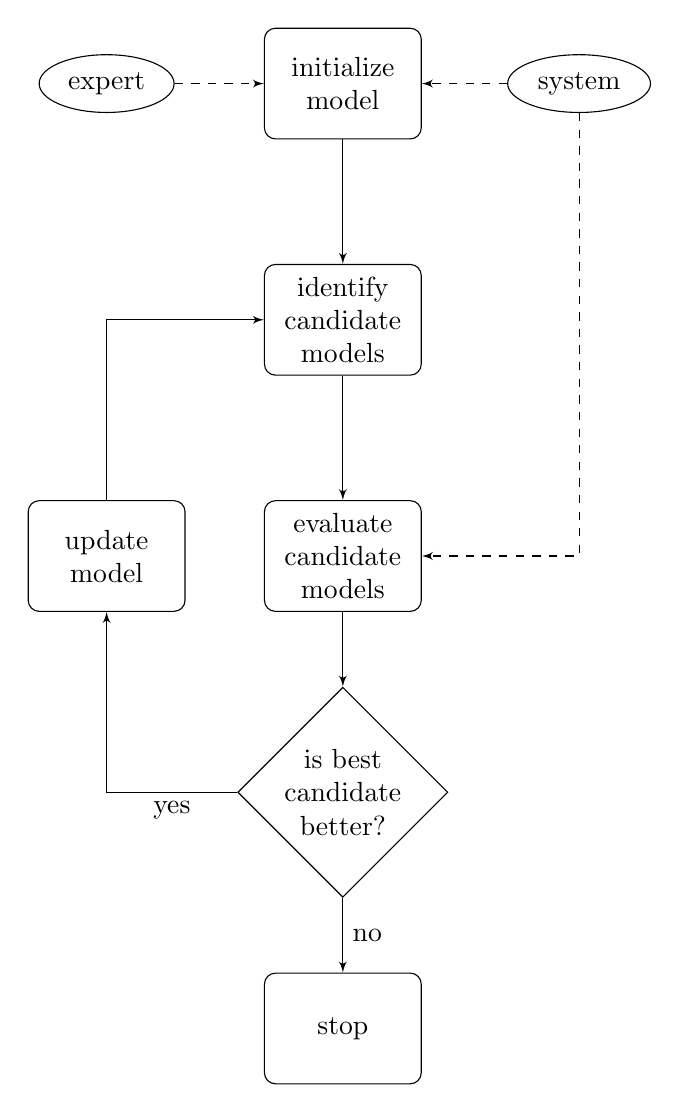
\begin{tikzpicture}[node distance = 3cm, auto]
% Define block styles
\tikzstyle{decision} = [diamond, draw, fill=white!20, 
    text width=4.5em, text badly centered, node distance=3cm, inner sep=0pt]
\tikzstyle{block} = [rectangle, draw, fill=white!20, 
    text width=5em, text centered, rounded corners, minimum height=4em]
\tikzstyle{line} = [draw, -latex']
\tikzstyle{cloud} = [draw, ellipse,fill=white!20, node distance=3cm,
    minimum height=2em]
    
    % Place nodes
    \node [block] (init) {initialize model};
    \node [cloud, left of=init] (expert) {expert};
    \node [cloud, right of=init] (system) {system};
    \node [block, below of=init] (identify) {identify candidate models};
    \node [block, below of=identify] (evaluate) {evaluate candidate models};
    \node [block, left of=evaluate, node distance=3cm] (update) {update model};
    \node [decision, below of=evaluate] (decide) {is best candidate better?};
    \node [block, below of=decide, node distance=3cm] (stop) {stop};
    % Draw edges
    \path [line] (init) -- (identify);
    \path [line] (identify) -- (evaluate);
    \path [line] (evaluate) -- (decide);
    \path [line] (decide) -| node [near start] {yes} (update);
    \path [line] (update) |- (identify);
    \path [line] (decide) -- node {no}(stop);
    \path [line,dashed] (expert) -- (init);
    \path [line,dashed] (system) -- (init);
    \path [line,dashed] (system) |- (evaluate);
\end{tikzpicture}
\end{center}








\begin{center}
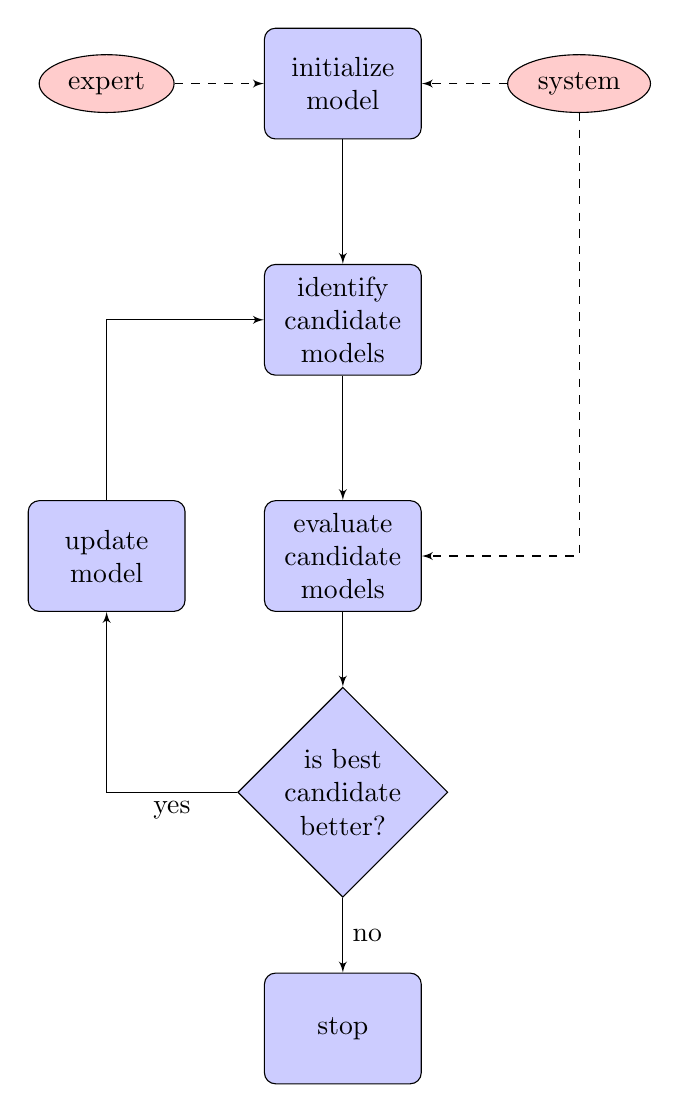
\begin{tikzpicture}[node distance = 3cm, auto]
% Define block styles
\tikzstyle{decision} = [diamond, draw, fill=blue!20, 
    text width=4.5em, text badly centered, node distance=3cm, inner sep=0pt]
\tikzstyle{block} = [rectangle, draw, fill=blue!20, 
    text width=5em, text centered, rounded corners, minimum height=4em]
\tikzstyle{line} = [draw, -latex']
\tikzstyle{cloud} = [draw, ellipse,fill=red!20, node distance=3cm, minimum height=2em]

    % Place nodes
    \node [block] (init) {initialize model};
    \node [cloud, left of=init] (expert) {expert};
    \node [cloud, right of=init] (system) {system};
    \node [block, below of=init] (identify) {identify candidate models};
    \node [block, below of=identify] (evaluate) {evaluate candidate models};
    \node [block, left of=evaluate, node distance=3cm] (update) {update model};
    \node [decision, below of=evaluate] (decide) {is best candidate better?};
    \node [block, below of=decide, node distance=3cm] (stop) {stop};
    % Draw edges
    \path [line] (init) -- (identify);
    \path [line] (identify) -- (evaluate);
    \path [line] (evaluate) -- (decide);
    \path [line] (decide) -| node [near start] {yes} (update);
    \path [line] (update) |- (identify);
    \path [line] (decide) -- node {no}(stop);
    \path [line,dashed] (expert) -- (init);
    \path [line,dashed] (system) -- (init);
    \path [line,dashed] (system) |- (evaluate);
\end{tikzpicture}
\end{center}










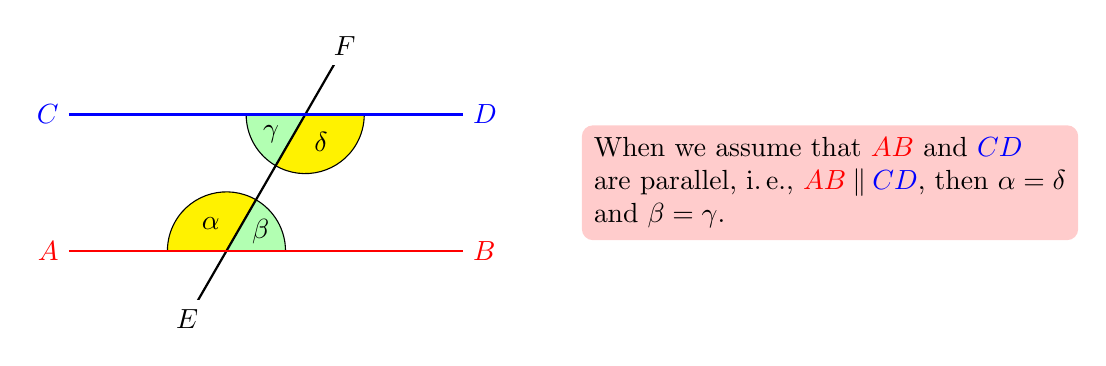
\begin{tikzpicture}
\draw[fill=yellow] (0,0) -- (60:.75cm) arc (60:180:.75cm);
\draw(120:0.4cm) node {$\alpha$};
\draw[fill=green!30] (0,0) -- (right:.75cm) arc (0:60:.75cm);
\draw(30:0.5cm) node {$\beta$};
\begin{scope}[shift={(60:2cm)}]
\draw[fill=green!30] (0,0) -- (180:.75cm) arc (180:240:.75cm);
\draw (30:-0.5cm) node {$\gamma$};
\draw[fill=yellow] (0,0) -- (240:.75cm) arc (240:360:.75cm);
\draw (-60:0.4cm) node {$\delta$};
\end{scope}
\begin{scope}[thick]
\draw (60:-1cm) node[fill=white] {$E$} -- (60:3cm) node[fill=white] {$F$};
\draw[red] (-2,0) node[left] {$A$} -- (3,0) node[right]{$B$};
\draw[blue,shift={(60:2cm)}] (-3,0) node[left] {$C$} -- (2,0) node[right]{$D$};

\draw[shift={(60:1cm)},xshift=4cm]
node [right,text width=6cm,rounded corners,fill=red!20,inner sep=1ex]
{
When we assume that $\color{red}AB$ and $\color{blue}CD$ are
parallel, i.\,e., ${\color{red}AB} \mathbin{\|} \color{blue}CD$,
then $\alpha = \delta$ and $\beta = \gamma$.
};
\end{scope}
\end{tikzpicture}








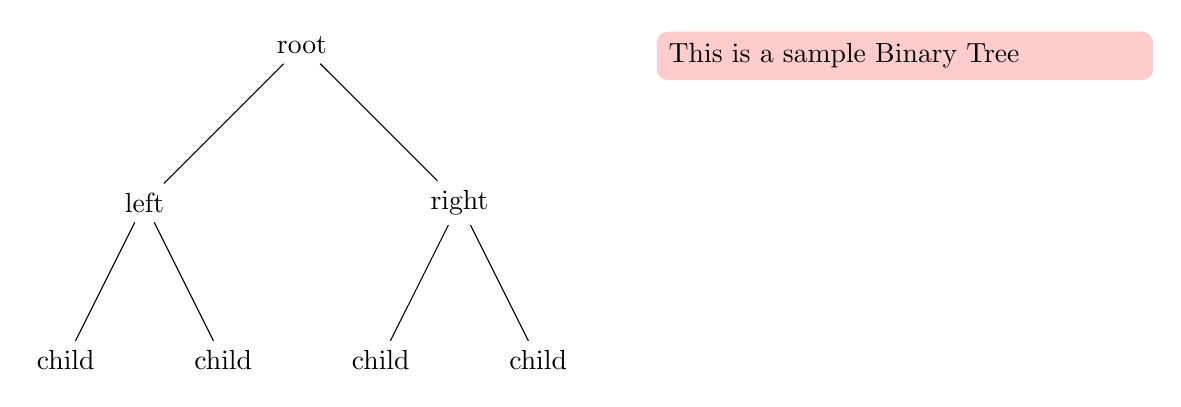
\begin{tikzpicture}[node distance=3cm,level distance=2cm]
\node {root} [sibling distance=4cm] 
child {node {left} [sibling distance=2cm]
	child {node {child}}
	child {node {child}}
}
child {node {right} [sibling distance=2cm]
	child {node {child}}
	child {node {child}}
};

\begin{scope}
\draw[shift={(60:1cm)},xshift=4cm,yshift=-1cm]
node [right,text width=6cm,rounded corners,fill=red!20,inner sep=1ex]
{
This is a sample Binary Tree
};
\end{scope}

\end{tikzpicture}








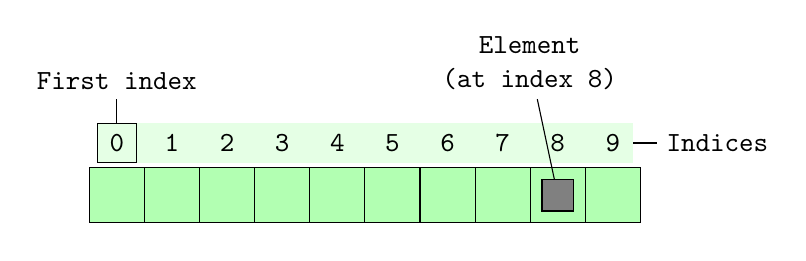
\begin{tikzpicture}[font=\ttfamily,
array/.style={matrix of nodes,nodes={draw, minimum size=7mm, fill=green!30},column sep=-\pgflinewidth, row sep=0.5mm, nodes in empty cells,
row 1/.style={nodes={draw=none, fill=none, minimum size=5mm}},
row 1 column 1/.style={nodes={draw}}}]

\matrix[array] (array) {
0 & 1 & 2 & 3 & 4 & 5 & 6 & 7 & 8 & 9\\
  &   &   &   &   &   &   &   &   &  \\};
\node[draw, fill=gray, minimum size=4mm] at (array-2-9) (box) {};

\begin{scope}[on background layer]
\fill[green!10] (array-1-1.north west) rectangle (array-1-10.south east);
\end{scope}

\draw (array-1-1.north)--++(90:3mm) node [above] (first) {First index};
\draw (array-1-10.east)--++(0:3mm) node [right]{Indices};
\node [align=center, anchor=south] at (array-2-9.north west|-first.south) (8) {Element\\ (at index 8)};
\draw (8)--(box);
%
\end{tikzpicture}
\\
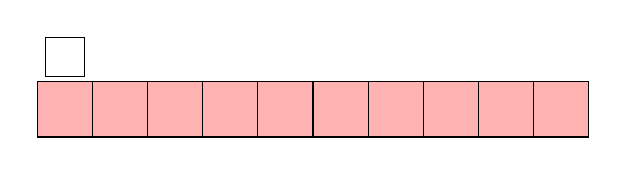
\begin{tikzpicture}[font=\ttfamily,
array/.style={matrix of nodes,nodes={draw, minimum size=7mm, fill=red!30},column sep=-\pgflinewidth, row sep=0.5mm, nodes in empty cells,
row 1/.style={nodes={draw=none, fill=none, minimum size=5mm}},
row 1 column 1/.style={nodes={draw}}}]

\matrix[array] (array) {
 &  &  &  &  &  &  &  &  & \\
 &   &   &   &   &   &   &   &   &  \\};
%
\end{tikzpicture}
\\
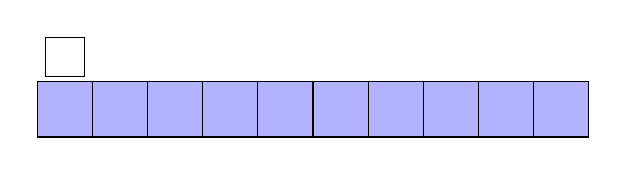
\begin{tikzpicture}[font=\ttfamily,
array/.style={matrix of nodes,nodes={draw, minimum size=7mm, fill=blue!30},column sep=-\pgflinewidth, row sep=0.5mm, nodes in empty cells,
row 1/.style={nodes={draw=none, fill=none, minimum size=5mm}},
row 1 column 1/.style={nodes={draw}}}]

\matrix[array] (array) {
 &  &  &  &  &  &  &  &  & \\
 &   &   &   &   &   &   &   &   &  \\};
%
\end{tikzpicture}






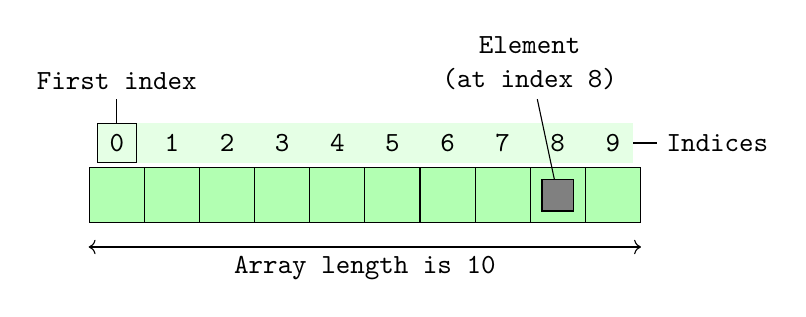
\begin{tikzpicture}[font=\ttfamily,
array/.style={matrix of nodes,nodes={draw, minimum size=7mm, fill=green!30},column sep=-\pgflinewidth, row sep=0.5mm, nodes in empty cells,
row 1/.style={nodes={draw=none, fill=none, minimum size=5mm}},
row 1 column 1/.style={nodes={draw}}}]

\matrix[array] (array) {
0 & 1 & 2 & 3 & 4 & 5 & 6 & 7 & 8 & 9\\
  &   &   &   &   &   &   &   &   &  \\};
\node[draw, fill=gray, minimum size=4mm] at (array-2-9) (box) {};

\begin{scope}[on background layer]
\fill[green!10] (array-1-1.north west) rectangle (array-1-10.south east);
\end{scope}

\draw[<->]([yshift=-3mm]array-2-1.south west) -- node[below] {Array length is 10} ([yshift=-3mm]array-2-10.south east);

\draw (array-1-1.north)--++(90:3mm) node [above] (first) {First index};
\draw (array-1-10.east)--++(0:3mm) node [right]{Indices};
\node [align=center, anchor=south] at (array-2-9.north west|-first.south) (8) {Element\\ (at index 8)};
\draw (8)--(box);
%
\end{tikzpicture}



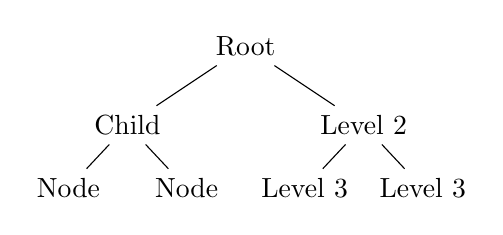
\begin{tikzpicture}[level distance=1.3cm,
   level 1/.style={sibling distance=3cm, level distance=1cm},
   level 2/.style={sibling distance=1.5cm, level distance=0.8cm}]
\node {Root}
   child {node {Child}
   child {node {Node}}
   child {node {Node}}
}
child {node {Level 2}
   child {node {Level 3}}
   child {node {Level 3}}
};
\end{tikzpicture}






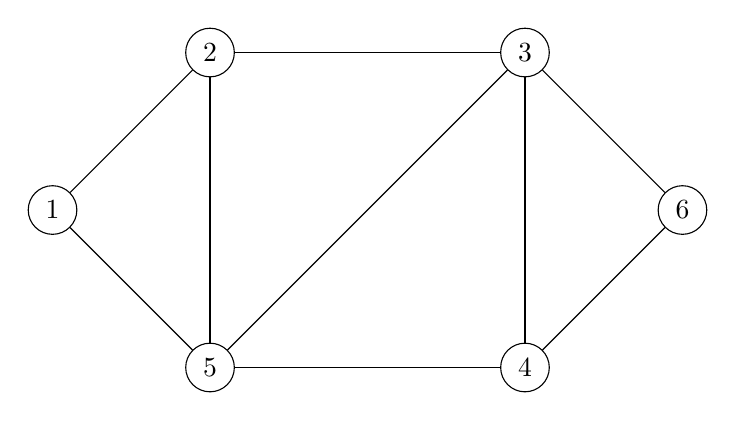
\begin{tikzpicture}
     \tikzstyle{node_style} = [circle,draw=black]
     \tikzstyle{edge_style} = [draw=black]
     \node[node_style] (v1) at (-2,2) {2};
     \node[node_style] (v2) at (2,2) {3};
     \node[node_style] (v3) at (4,0) {6};
     \node[node_style] (v4) at (2,-2) {4};
     \node[node_style] (v5) at (-2,-2) {5};
     \node[node_style] (v6) at (-4,0) {1};
     \draw[edge_style]  (v1) edge (v2);
     \draw[edge_style]  (v2) edge (v3);
     \draw[edge_style]  (v3) edge (v4);
     \draw[edge_style]  (v4) edge (v5);
     \draw[edge_style]  (v5) edge (v6);
     \draw[edge_style]  (v6) edge (v1);
     \draw[edge_style]  (v5) edge (v1);
     \draw[edge_style]  (v5) edge (v2);
     \draw[edge_style]  (v4) edge (v2);
\end{tikzpicture}






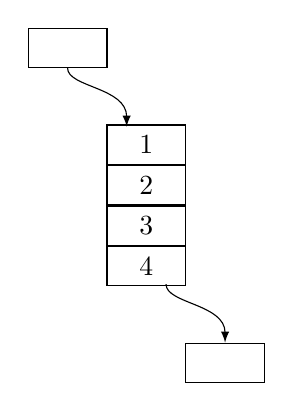
\begin{tikzpicture}[draw, minimum width=1cm, minimum height=0.5cm]
    \node[draw] (in) at (-1,2) {};
    \node[draw] (out) at (1,-2) {};
    \matrix (queue)[matrix of nodes, nodes={draw, nodes={draw}}, nodes in empty cells]
    {
       1 \\ 2 \\ 3 \\ 4 \\
    };

    \draw[-latex] (0.25,-1) .. controls (0.25,-1.25) and (1,-1.25) .. (out.north);
    \draw[-latex] (in.south) .. controls (-1, 1.5) and (-0.25,1.5) .. (-0.25,1);
\end{tikzpicture}









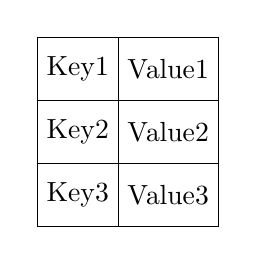
\begin{tikzpicture} [nodes={minimum width=0.8cm, minimum height=0.8cm},
         row sep=-\pgflinewidth, column sep=-\pgflinewidth]
   \matrix (hash)[matrix of nodes, nodes={draw, anchor=center}]
         {
       Key1 & Value1 \\
       Key2 & Value2 \\
       Key3 & Value3 \\
    };
\end{tikzpicture}



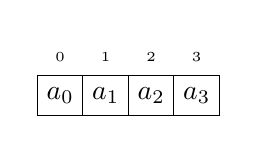
\begin{tikzpicture} [nodes in empty cells,
      nodes={minimum width=0.5cm, minimum height=0.5cm},
      row sep=-\pgflinewidth, column sep=-\pgflinewidth]
      border/.style={draw}
    
      \matrix(vector)[matrix of nodes,
          row 1/.style={nodes={draw=none, minimum width=0.3cm}},
          nodes={draw}]
      {
          \tiny{0} & \tiny{1} & \tiny{2} & \tiny{3}\\
          $a_{0}$ & $a_{1}$ & $a_{2}$ & $a_{3}$\\
      };
\end{tikzpicture}




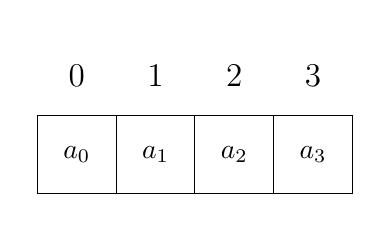
\begin{tikzpicture} [nodes in empty cells,
      nodes={minimum width=1cm, minimum height=1cm},
      row sep=-\pgflinewidth, column sep=-\pgflinewidth]
      border/.style={draw}
    
      \matrix(vector)[matrix of nodes,
          row 1/.style={nodes={draw=none, minimum width=0.3cm}},
          nodes={draw}]
      {
      	   
          \large{0} & \large{1} & \large{2} & \large{3} \\
          $a_{0}$ & $a_{1}$ & $a_{2}$ & $a_{3}$ \\
      };
\end{tikzpicture}





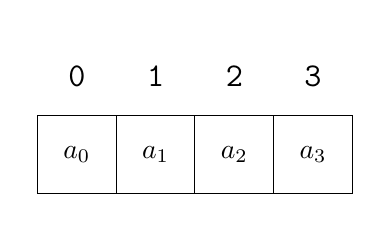
\begin{tikzpicture} [nodes in empty cells,
      nodes={minimum width=1cm, minimum height=1cm},
      row sep=-\pgflinewidth, column sep=-\pgflinewidth]
      border/.style={draw}
    
      \matrix(vector)[matrix of nodes,
          row 1/.style={nodes={draw=none, minimum width=0.3cm}},
          nodes={draw}]
      {
      	   
          \ttfamily\large{0} & \ttfamily\large{1} & \ttfamily\large{2} & \ttfamily\large{3} \\
          $a_{0}$ & $a_{1}$ & $a_{2}$ & $a_{3}$ \\
      };
\end{tikzpicture}







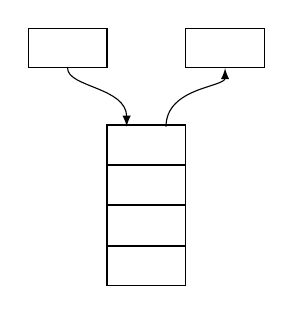
\begin{tikzpicture}[draw, minimum width=1cm, minimum height=0.5cm]
    \node[draw] (in) at (-1,2) {};
    \node[draw] (out) at (1,2) {};
    \matrix (queue)[matrix of nodes, nodes={draw, nodes={draw}}, nodes in empty cells]
    {
       \\ \\ \\ \\
    };

    \draw[-latex] (0.25,1) .. controls (0.25,1.5) and (1,1.5) .. (out.south);
    \draw[-latex] (in.south) .. controls (-1, 1.5) and (-0.25,1.5) .. (-0.25,1);
\end{tikzpicture}








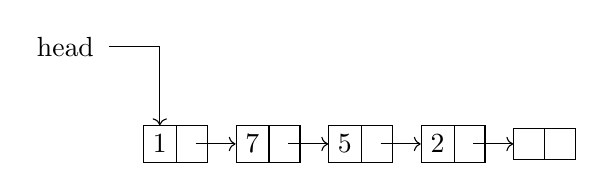
\begin{tikzpicture}[every node/.style={rectangle split, rectangle split parts=2, rectangle split horizontal}, node distance=1em, start chain, 
 every join/.style={->, shorten <=-4.5pt}]

 \node[draw, on chain, join] { 1  };
 \node[draw, on chain, join] { 7  };
 \node[draw, on chain, join] { 5  };
 \node[draw, on chain, join] { 2  };
 \node[draw, on chain, join] {};
 \chainlabel{chain-1.one north}{head};
\end{tikzpicture}  

{
.
\\
\\
}

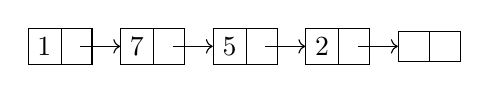
\begin{tikzpicture}[every node/.style={rectangle split, rectangle split parts=2, rectangle split horizontal}, node distance=1em, start chain, 
 every join/.style={->, shorten <=-4.5pt}]

 \node[draw, on chain, join] { 1  };
 \node[draw, on chain, join] { 7  };
 \node[draw, on chain, join] { 5  };
 \node[draw, on chain, join] { 2  };
 \node[draw, on chain, join] {};
%\chainlabel{chain-1.one north}{head};
\end{tikzpicture}  








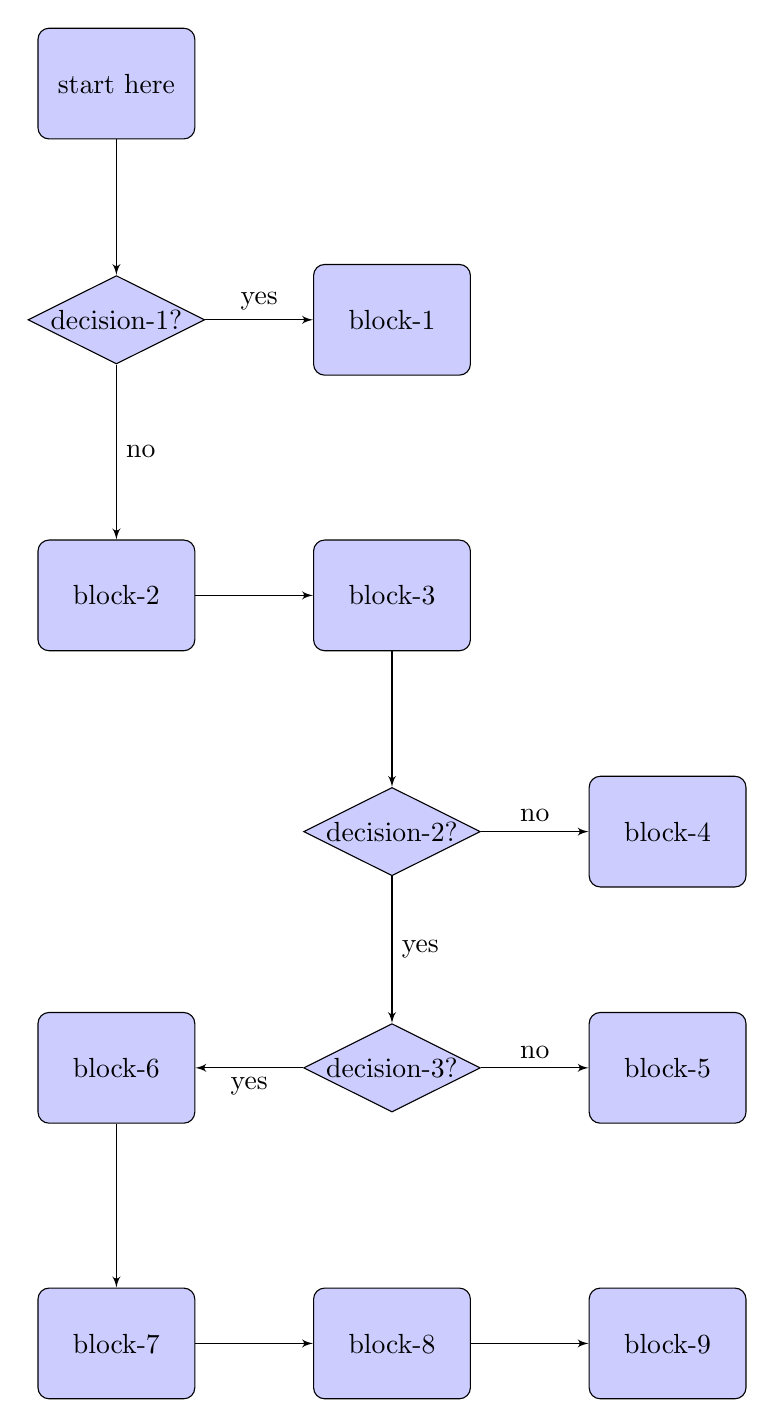
\begin{tikzpicture}[node distance=3.5cm, auto]
 \tikzstyle{decision} = [ diamond, aspect=2, draw, fill=blue!20, text width=5em, text badly centered, node distance=3cm, inner sep=0pt ]
\tikzstyle{block} = [ rectangle, draw, fill=blue!20, text width=5em, text centered, rounded corners, minimum height=4em ]
\tikzstyle{line} = [ draw, -latex' ]
% place nodes
\node [block] (init) {start here} ;
\node [decision, below of=init] (decision-1) {decision-1?} ;
\node [block, right of=decision-1] (block-1) {block-1} ;
\node [block, below of=decision-1] (block-2) {block-2} ;
\node [block, right of=block-2] (block-3) {block-3} ;
\node [decision, below of=block-3] (decision-2) {decision-2?} ;
\node [block, right of=decision-2] (block-4) {block-4} ;
\node [decision, below of=decision-2] (decision-3) {decision-3?} ;
\node [block, left of=decision-3] (block-6) {block-6} ;
\node [block, right of=decision-3] (block-5) {block-5} ;
\node [block, below of=block-6] (block-7) {block-7} ;
\node [block, right of=block-7] (block-8) {block-8} ;
\node [block, right of=block-8] (block-9) {block-9} ;


% draw edges
\path [line] (init) -- (decision-1) ;
\path [line] (decision-1) -- node {yes}(block-1) ;
\path [line] (decision-1) -- node {no}(block-2) ;
\path [line] (block-2) -- (block-3) ;
\path [line] (block-3) -- (decision-2) ;
\path [line] (decision-2) -- node {no}(block-4) ;
\path [line] (decision-2) -- node {yes}(decision-3) ;
\path [line] (decision-3) -- node {yes}(block-6) ;
\path [line] (decision-3) -- node {no}(block-5) ;
\path [line] (block-6) -- (block-7) ;
\path [line] (block-7) -- (block-8) ;
\path [line] (block-8) -- (block-9) ;
 
\end{tikzpicture}


{
.
\newline
\newline
\newline
}

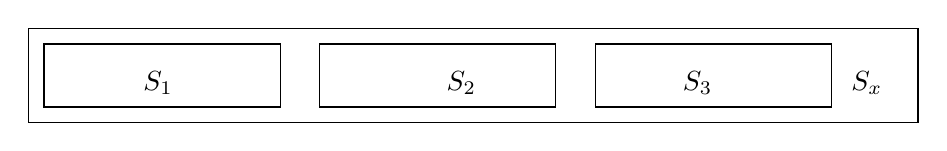
\begin{tikzpicture}[shift={(1,1)},local bounding box=A]
\draw (0,0) rectangle (11.3,1.2);
\draw (0.2,0.2) rectangle (3.2,1);
\draw (3.7,0.2) rectangle (6.7,1);
\draw (7.2,0.2) rectangle (10.2,1);
\node[scale=1] at (1.65,0.5) {$S_{1}$};
\node[scale=1] at (5.5,0.5) {$S_{2}$};
\node[scale=1] at (8.5,0.5) {$S_{3}$};
\node[scale=1] at (10.65,0.5) {$S_{x}$};
\end{tikzpicture}

{
.
\newline
\newline
\newline
}

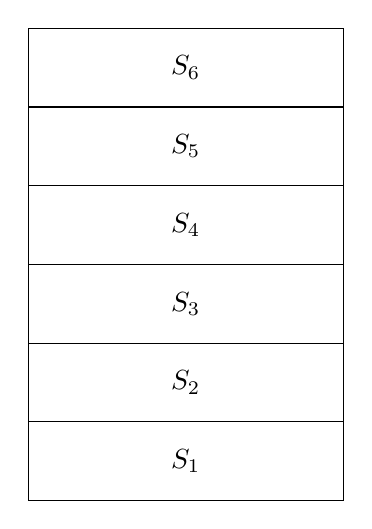
\begin{tikzpicture}
\draw (0,0) rectangle (4,6);

\draw (0,0) rectangle (4,1);
\draw (0,1) rectangle (4,1);
\draw (0,2) rectangle (4,1);
\draw (0,3) rectangle (4,1);
\draw (0,4) rectangle (4,1);
\draw (0,5) rectangle (4,1);
\draw (0,6) rectangle (4,1);


\node[scale=1] at (2,0.5) {$S_{1}$};
\node[scale=1] at (2,1.5) {$S_{2}$};
\node[scale=1] at (2,2.5) {$S_{3}$};
\node[scale=1] at (2,3.5) {$S_{4}$};
\node[scale=1] at (2,4.5) {$S_{5}$};
\node[scale=1] at (2,5.5) {$S_{6}$};
\end{tikzpicture}





{
.
\newline
\newline
\newline
}




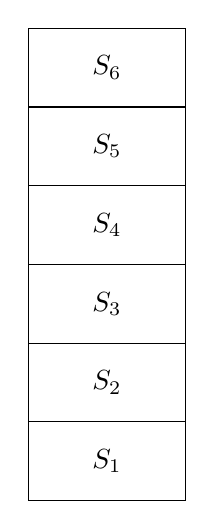
\begin{tikzpicture}
\draw (0,0) rectangle (2,6);

\draw (0,0) rectangle (2,1);
\draw (0,1) rectangle (2,1);
\draw (0,2) rectangle (2,1);
\draw (0,3) rectangle (2,1);
\draw (0,4) rectangle (2,1);
\draw (0,5) rectangle (2,1);
\draw (0,6) rectangle (2,1);


\node[scale=1] at (1,0.5) {$S_{1}$};
\node[scale=1] at (1,1.5) {$S_{2}$};
\node[scale=1] at (1,2.5) {$S_{3}$};
\node[scale=1] at (1,3.5) {$S_{4}$};
\node[scale=1] at (1,4.5) {$S_{5}$};
\node[scale=1] at (1,5.5) {$S_{6}$};
\end{tikzpicture}




{
.
\newline
\newline
\newline
}




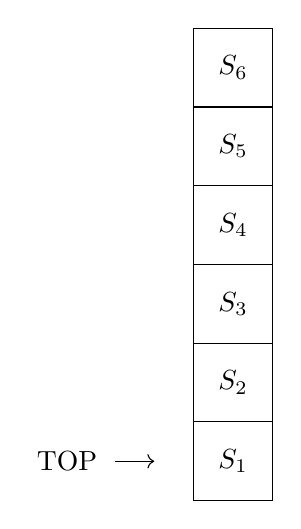
\begin{tikzpicture}
\draw (0,0) rectangle (1,6);

\draw (0,0) rectangle (1,1);
\draw (0,1) rectangle (1,1);
\draw (0,2) rectangle (1,1);
\draw (0,3) rectangle (1,1);
\draw (0,4) rectangle (1,1);
\draw (0,5) rectangle (1,1);
\draw (0,6) rectangle (1,1);

\draw [->] (-1,0.5) -- (-.5,0.5) node[left, xshift=-6mm] {TOP};


\node[scale=1] at (0.5,0.5) {$S_{1}$};
\node[scale=1] at (0.5,1.5) {$S_{2}$};
\node[scale=1] at (0.5,2.5) {$S_{3}$};
\node[scale=1] at (0.5,3.5) {$S_{4}$};
\node[scale=1] at (0.5,4.5) {$S_{5}$};
\node[scale=1] at (0.5,5.5) {$S_{6}$};
\end{tikzpicture}




{
.
\newline
\newline
\newline
}




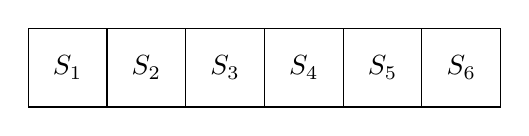
\begin{tikzpicture}
\draw (0,0) rectangle (6,1);

\draw (0,0) rectangle (1,1);
\draw (1,0) rectangle (1,1);
\draw (2,0) rectangle (1,1);
\draw (3,0) rectangle (1,1);
\draw (4,0) rectangle (1,1);
\draw (5,0) rectangle (1,1);
\draw (6,0) rectangle (1,1);


\node[scale=1] at (0.5,0.5) {$S_{1}$};
\node[scale=1] at (1.5,0.5) {$S_{2}$};
\node[scale=1] at (2.5,0.5) {$S_{3}$};
\node[scale=1] at (3.5,0.5) {$S_{4}$};
\node[scale=1] at (4.5,0.5) {$S_{5}$};
\node[scale=1] at (5.5,0.5) {$S_{6}$};
\end{tikzpicture}




{
.
\newline
\newline
\newline
}




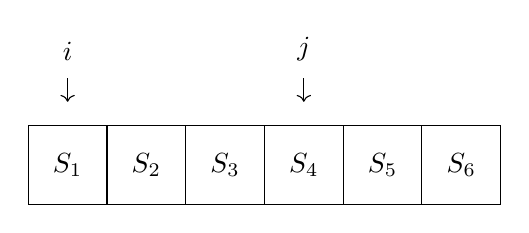
\begin{tikzpicture}
\draw (0,0) rectangle (6,1);

\draw (0,0) rectangle (1,1);
\draw (1,0) rectangle (1,1);
\draw (2,0) rectangle (1,1);
\draw (3,0) rectangle (1,1);
\draw (4,0) rectangle (1,1);
\draw (5,0) rectangle (1,1);
\draw (6,0) rectangle (1,1);

\draw [->] (0.5,1.6) -- (0.5,1.3) node[above, yshift=4mm] {$i$};

\draw [->] (3.5,1.6) -- (3.5,1.3) node[above, yshift=4mm] {$j$};

\node[scale=1] at (0.5,0.5) {$S_{1}$};
\node[scale=1] at (1.5,0.5) {$S_{2}$};
\node[scale=1] at (2.5,0.5) {$S_{3}$};
\node[scale=1] at (3.5,0.5) {$S_{4}$};
\node[scale=1] at (4.5,0.5) {$S_{5}$};
\node[scale=1] at (5.5,0.5) {$S_{6}$};
\end{tikzpicture}








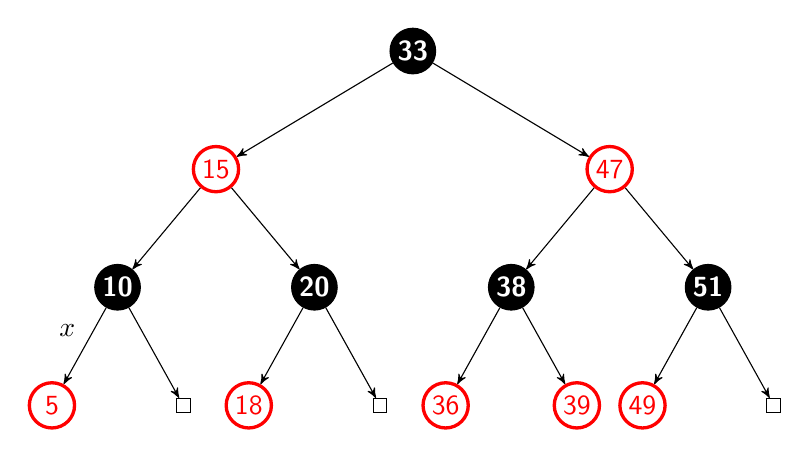
\begin{tikzpicture}[->,>=stealth',level/.style={sibling distance = 5cm/#1,
  level distance = 1.5cm}] 
  \tikzset{
  treenode/.style = {align=center, inner sep=0pt, text centered,
    font=\sffamily},
  arn_n/.style = {treenode, circle, white, font=\sffamily\bfseries, draw=black,
    fill=black, text width=1.5em},% arbre rouge noir, noeud noir
  arn_r/.style = {treenode, circle, red, draw=red, 
    text width=1.5em, very thick},% arbre rouge noir, noeud rouge
  arn_x/.style = {treenode, rectangle, draw=black,
    minimum width=0.5em, minimum height=0.5em}% arbre rouge noir, nil
}


\node [arn_n] {33}
    child{ node [arn_r] {15} 
            child{ node [arn_n] {10} 
            	child{ node [arn_r] {5} edge from parent node[above left]
                         {$x$}} %for a named pointer
							child{ node [arn_x] {}}
            }
            child{ node [arn_n] {20}
							child{ node [arn_r] {18}}
							child{ node [arn_x] {}}
            }                            
    }
    child{ node [arn_r] {47}
            child{ node [arn_n] {38} 
							child{ node [arn_r] {36}}
							child{ node [arn_r] {39}}
            }
            child{ node [arn_n] {51}
							child{ node [arn_r] {49}}
							child{ node [arn_x] {}}
            }
		}
; 
\end{tikzpicture}






















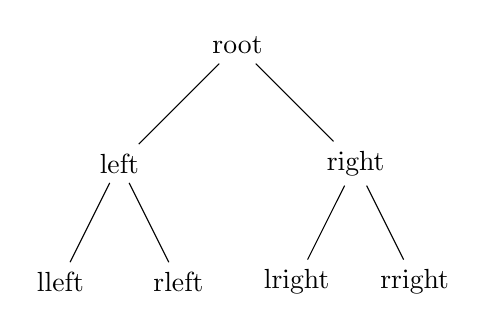
\begin{tikzpicture}[level distance=1.5cm,
  level 1/.style={sibling distance=3cm},
  level 2/.style={sibling distance=1.5cm}]
  \node {root}
    child {node {left}
      child {node {lleft}}
      child {node {rleft}}
    }
    child {node {right}
    child {node {lright}}
      child {node {rright}}
    };
\end{tikzpicture}







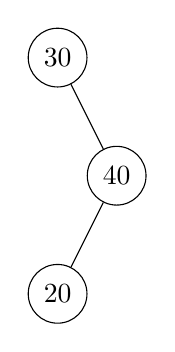
\begin{tikzpicture}
\node[circle,draw](z){$30$}
  child[missing]{}
  child{ node[circle,draw]{40} 
	  child{ node[circle,draw] {20} } 
	  child[missing] 
  };
\end{tikzpicture}










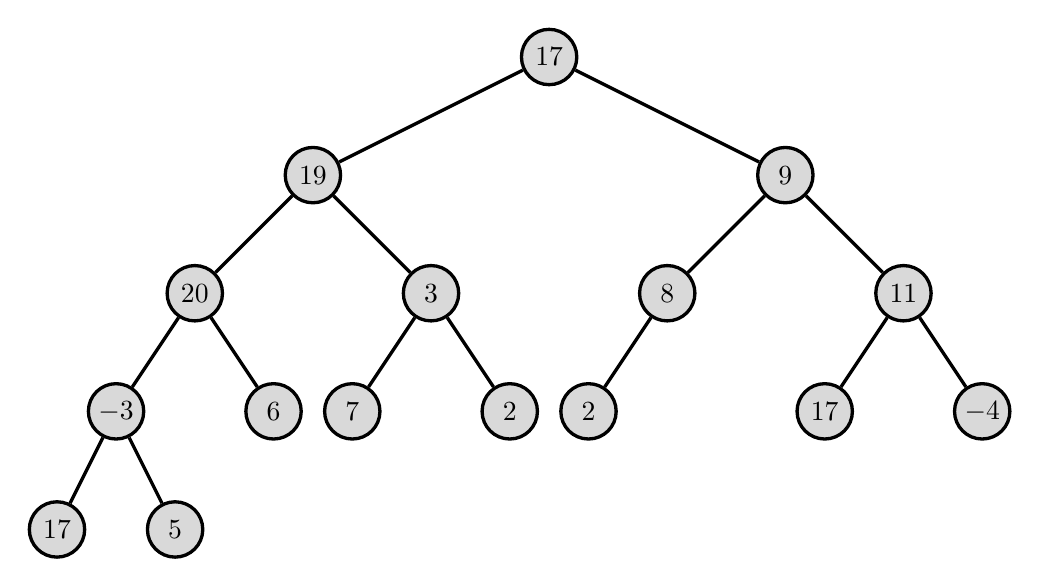
\begin{tikzpicture}[very thick,level/.style={sibling distance=60mm/#1}]
\tikzstyle{vertex}=[draw,fill=black!15,circle,minimum size=20pt,inner sep=1pt]
\node [vertex] (r){$17$}
  child {
	    node [vertex] (a) {$19$}
	    child {
		      node [vertex] {$20$}
		      child {
			        node [vertex] {$-3$}
			        child {node [vertex] {$17$}}
			        child {node [vertex] {$5$}}
		      }
		      child {node [vertex] {$6$}}
	    }
	    child {
		      node [vertex] {$3$}
		      child {node [vertex] {$7$}}
		      child {node [vertex] {$2$}}
	    }
  }
  child {
	    node [vertex] {$9$}
	    child {
		      node [vertex] {$8$}
		      child {node [vertex] {$2$}}
		      child [missing] {} 
	    }
	    child {
		      node [vertex] {$11$}
		      child {node [vertex] {$17$}}
		      child {node [vertex] {$-4$}}
	    }
  };
\end{tikzpicture}












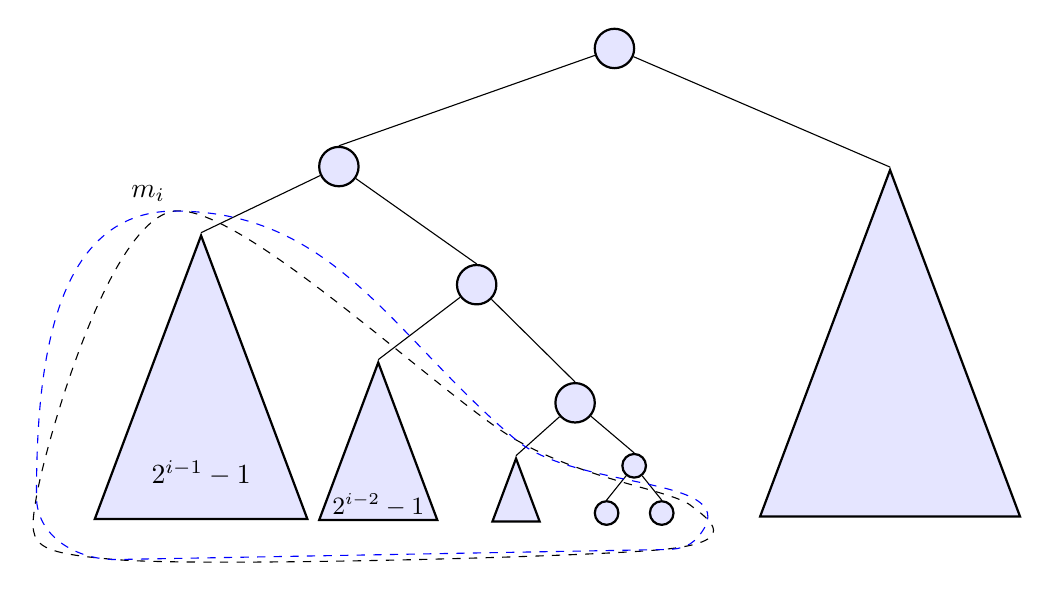
\begin{tikzpicture}[
  inner/.style={fill = light blue,circle,draw,thick,minimum width=5mm,inner sep=0},
  small inner/.style={inner,minimum width = 3mm},
  triangle/.style={fill = light blue,isosceles triangle,draw=,thick,shape border rotate=90,isosceles triangle stretches=true, minimum height=20mm,minimum width=15mm,inner sep=0,yshift={-10mm}},
  small triangle/.style={triangle, minimum height = 8mm, minimum width = 6mm },
  large triangle/.style={triangle,minimum width = 27mm,minimum height=36mm,yshift={-11mm}},
  very large triangle/.style={triangle,minimum width = 33mm,minimum height=44mm,yshift={-11mm}},
  level 1/.style={sibling distance=70mm},
  level 2/.style={sibling distance=35mm},
  level 3/.style={sibling distance=25mm},
  level 4/.style={sibling distance=25mm},
  level 4/.style={sibling distance=15mm},
  level 5/.style={sibling distance=7mm},
]
  \colorlet{light blue}{blue!10}
  \node[inner] {}
     [child anchor=north]
    child {node[inner] {}
        child {node[large triangle,yshift={-3mm}] (a) {$2^{i-1}-1$}}
        child {node[inner,yshift={0mm}] {}
            child{node[triangle,font=\small,yshift={-3mm}] (b) {$2^{i-2}-1$}}
            child{node[inner,yshift={0mm}] {}
                child{node[small triangle,font=\fontsize{6}{3},yshift={12mm}] (c) {}}
                child{node[small inner,yshift={7mm}]{}
                    child{node[small inner,yshift={9mm}] (d) {}}
                    child{node[small inner,yshift={9mm}] (e) {}}
                }
            }
        }
    }
    child {node[very large triangle ,yshift={-12mm}] {}};

\coordinate (A) at ([yshift=2.5cm,xshift=.5cm]a.north west);
\coordinate (B) at ([yshift=.2cm]c.north);
\coordinate (C) at ([xshift=.2cm,yshift=.1cm]e.east);
\coordinate (D) at ([xshift=.3cm,yshift=-.3cm]e.east);
\coordinate (E) at ([yshift=-.3cm]e.south);
\coordinate (F) at ([xshift=-.5cm,yshift=-.5cm]a.south west);
\coordinate (G) at ([xshift=-1.5cm,yshift=.3cm]a.south west);

\draw[dashed] plot[smooth cycle] coordinates {(A) (B) (C) (E) (F) (G)};

\draw [dashed,blue] (A) to[out=0,in=140]
      (B) to[out=320,in=50]
      (D) to[out=230,in=0] 
      (E) to
      (F) to[out=180,in=270]
      (G) to[out=90,in=180] (A);

\node at (A) [above  left] {\( m_i \)};
\end{tikzpicture}

















\end{document}